\chapterbegin{Red inal�mbrica}
\label{chp:redInalambrica}
\minitoc

\section{Introducci�n}

La red inal�mbrica es la parte de este \ac{TFG} que engloba al nodo y al concentrador (v�ase figura \ref{fig:esquemaGeneral}). En este cap�tulo se detallan las caracter�sticas y funcionamiento de cada una de las partes.

\section{Nodo}



\subsection*{Introducci�n}

La aplicaci�n implementa el dispositivo de la red, que le permite conectarse a la red creada por el concentrador. El sensor peri�dicamente env�a reportes de datos en intervalos configurados por el concentrador y este responde con mensajes de rastreo.

\subsection*{Arquitectura Hardware}

\subsection*{ARM Cortex M0 (N�cleo radio)}
El n�cleo \ac{CM0} en el CC1350 es responsable de la interfaz audio, y traduce complejas instrucciones del n�cleo \ac{CM3}  en bits que son enviados a trav�s del enlace radio.  Para el protocolo TI 15.4-Stack, el \ac{CM0} implementa la capa \ac{PHY} de la pila de protocolos. \\

El \textit{firmware} del n�cleo de radio no est� destinado a ser usado o modificado por la aplicaci�n del desarrollador.

\begin{figure}[H]
	\centering
	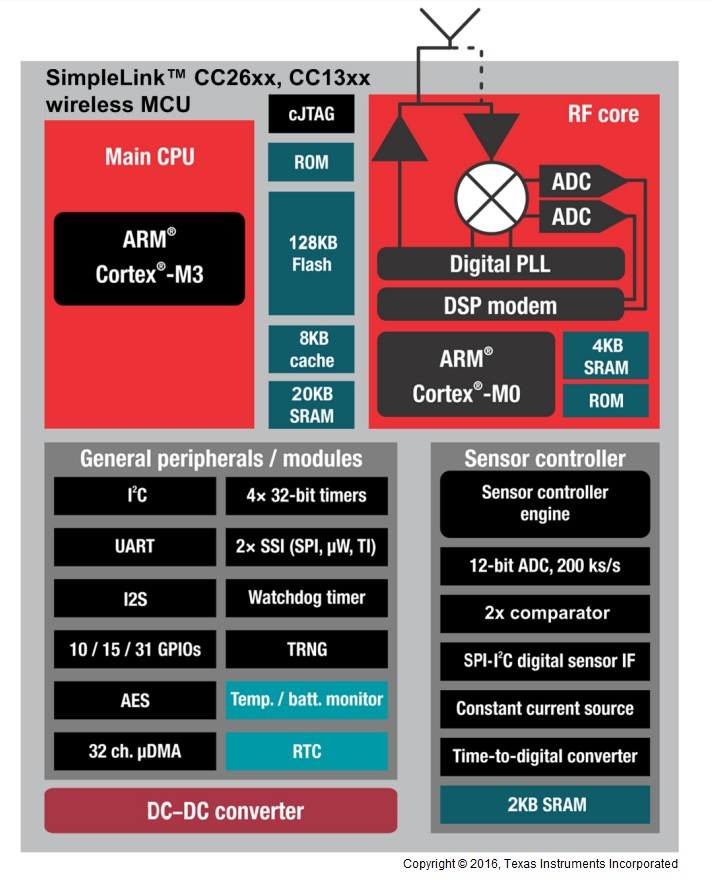
\includegraphics[width=0.5\textwidth]{graphs/fig-simplelink-block-diagram.jpeg}
	\caption{Diagrama de bloques de Simplelink\TM CC13x0}
	\label{fig:diagramaBloquesSimpleLink}
\end{figure}

\subsubsection*{ARM Cortex M3 (N�cleo del sistema)}

El n�cleo \ac{CM3} est� dise�ado para ejecutar la pila del protocolo inal�mbrico desde la capa de enlace hasta la capa de aplicaci�n de usuario. La capa de enlace act�a como interfaz del n�cleo de radio c�mo un m�dulo software llamado \textit{RF driver}.

\subsubsection*{Flash, RAM y perif�ricos}

El CC1350 contiene en el sistema 128KB de memoria flash programable, 20KB de SRAM, y un amplio rango de perif�ricos. La memora flash se divide en partes que se pueden borrar de 4KB. El CC1350 tambi�n contiene 8kB de cach� SRAM que puede ser utilizada para extender la capacidad de la RAM o puede funcionar como una cach� normal para incrementar el rendimiento de la aplicaci�n. Otros perif�ricos incluidos son UART, I2C, I2S, AES, TRNG, temperatura y monitor de la bater�a.



\subsection*{TI-RTOS}

TI-RTOS es un entorno operativo para proyectos TI 15.4-Stack en dispositivos CC1350. El kernel TI-RTOS es una versi�n adaptada del kernel SYS/BIOS y funciona como un sistema operativo con controladores en tiempo real, con prioridades, multitarea y herramientas para la sincronizaci�n y planificaci�n.

% TODO Completar esta secci�n

\subsection*{Arquitectura de la aplicaci�n}

En la figura \ref{fig:fig-example-application-block-diagram} se muestra el diagrama de bloques de la aplicaci�n del nodo.  

\begin{figure}[h]
	\centering
	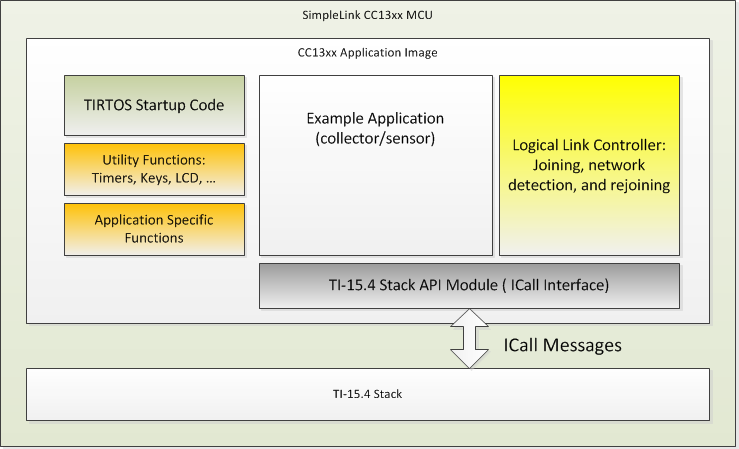
\includegraphics[width=0.8\textwidth]{graphs/fig-example-application-block-diagram}
	\caption{Diagrama de bloques de la aplicaci�n}
	\label{fig:fig-example-application-block-diagram}
\end{figure}


\begin{description}
	\item[Aplicaci�n:] Este bloque contiene la l�gica espec�fica de la aplicaci�n a desarrollar.
	\item[Controlador de l�gica de enlace:] Implementa varias funciones espec�ficas del IEEE 802.15.4 o Wi-SUN (para una configuraci�n \textit{frequency-hopping}) para formaci�n, conexi�n y reconexi�n de la red. 
	\item[Inicio de TI-RTOS:] Inicializa la aplicaci�n.
	\item[Funciones �tiles] Provee varias utilidades para usar LCD, temporizadores, botones y m�s.
	\item[Funciones espec�ficas:] Implementa funciones como guardado de datos, y provee una interfaz para gestionar pulsaciones botones o mostrar informaci�n esencial en un LCD.
	\item[TI 15.4-Stack API (API MAC Module):] Este m�dulo proporciona una interfaz para gesti�n y los servicios de datos del 802.15.4 stack mediante el m�dulo \ac{ICall}.
\end{description}

\subsection*{Funci�n de inicio}

La funci�n \textit{main()} dentro del archivo \textit{main.c} es el punto de inicio de la ejecuci�n de la aplicaci�n. En este punto los componentes relaciones con la placa son inicializados. Las tareas se configuran en eta funci�n, inicializando los par�metros necesarios como su prioridad y su tama�o en la pila. En el paso final, las interrupciones se habilitan y el planificador \textit{SYS/BIOS} se inicia llamando a \textit{BIOS\_start()}.


\subsection*{Arquitectura general de la aplicaci�n}

Esta secci�n describe como la tarea de la aplicaci�n esta estructura en m�s detalle. 

\subsubsection*{Funci�n de inicio de la aplicaci�n}

\begin{wrapfigure}{r}{0.4\textwidth}
	\begin{center}
		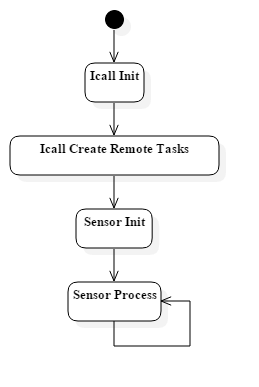
\includegraphics[width=0.4\textwidth]{graphs/TaskFxn.png}
	\end{center}
	\caption{Diagrama de estados de la funci�n de inicio}
\end{wrapfigure}

Despu�s de que la tarea sea construida y el planificador \textit{SYS/BIOS} se inicie, la funci�n que se le pasa durante la construcci�n de la tarea es ejecutada cuando la tarea est� lista.\\

Las funciones de gesti�n de la energ�a son inicializadas aqu� y el m�dulo \ac{ICall} se inicia con la funci�n \textit{ICall\_init()}. La direcci�n IEEE address (programada por TI) es obtenida desde la memoria flash. La tarea de la aplicaci�n (Aplicaci�n Sensor) es inicializada y ejecutada.

\textit{Sensor\_init()} establece varios par�metros de configuraci�n, as� como:

\begin{itemize}
	\item Inicializa las estructuras para los datos
	\item Inicializa el TI 15.4-Stack
	\item Configura la seguridad y el \textit{Logical Link Controller}
	\item Registra las funciones de retorno MAC
\end{itemize} 

\subsection*{Tarea principal}

Despu�s de la funci�n de inicializaci�n, la tarea entra en un bucle infinito ejecutando siempre las mismas tareas,  se puede ver en la figura

\begin{figure}[h]
	\centering
	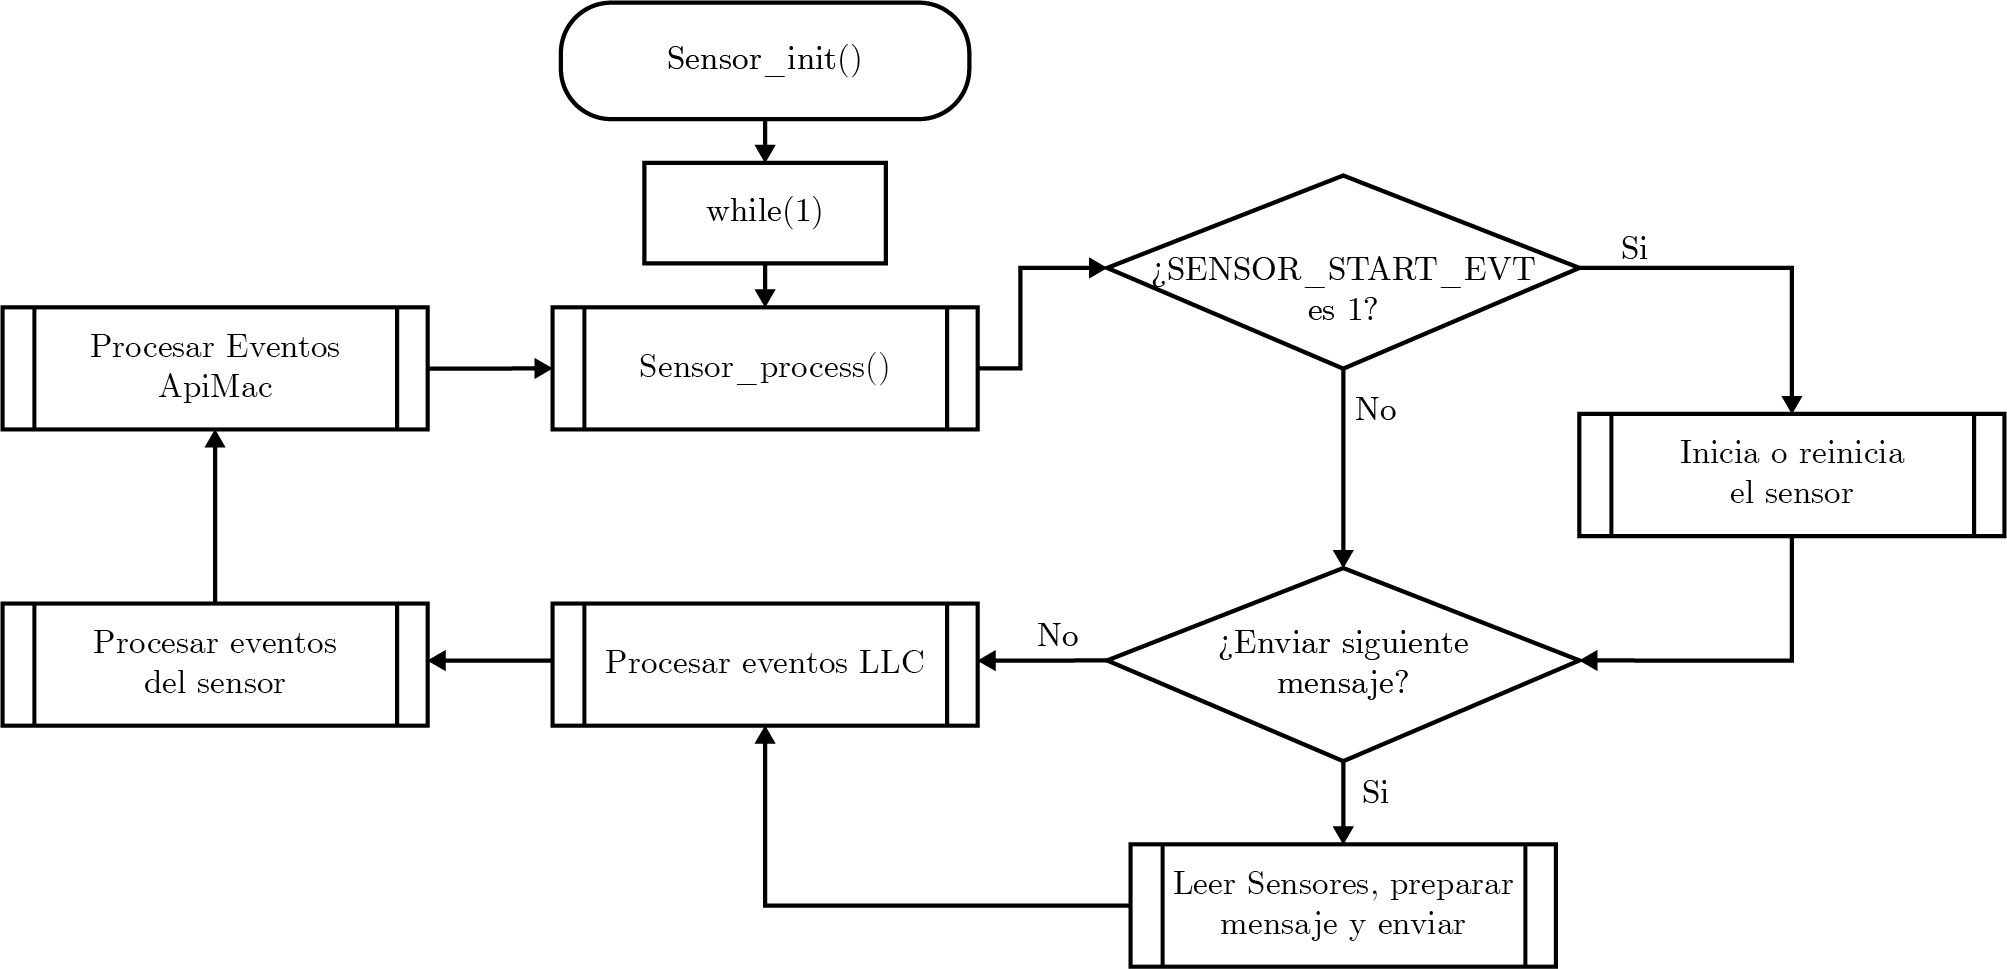
\includegraphics[width=0.8\textwidth]{graphs/fig-sensor-task-flow-chart}
	\caption{Flujo de la aplicaci�n}
	\label{fig:fig-sensor-task-flow-chart}
\end{figure}


\subsection*{Web f�sica}

La librer�a \ac{uBle} permite a la aplicaci�n enviar un paquete en modo \textit{broadcast} a todos los usuarios que est�n en el radio de acci�n del dispositivo. Este paquete de datos es el que utilizamos para notificar a los usuarios con la informaci�n de la web f�sica.\\

Los paquetes bluetooth usan la trama \textit{Eddystone-URL}, estas forman parte del n�cleo de la web f�sica. Una vez el usuario la decodifica la trama podr� acceder a la URL si tiene conexi�n a internet.\\

\subsubsection*{Especificaciones  de la trama}

\begin{table}
	\centering
	\begin{tabular}{|c|c|c|}
		\hline 
		Byte offset & Campo & Descripci�n \\ 
		\hline 
		0 & Tipo de trama & valor = 0x10 \\ 
		\hline 
		1 & Potencia TX & Potencia de TX calibrara a 0 m \\ 
		\hline 
		2 & Prefijo de la URL & Prefijo de la web \\ 
		\hline 
		3+ & URL codificada & Longitud de 1-17 bytes \\ 
		\hline 
	\end{tabular} 
	\caption{Formato de la trama \textit{Eddystone-URL}}
	\label{tab:formatoEddystone}
\end{table}

\begin{description}
	\item[Potencia TX] La potencia de transmisi�n es la potencia recibida a 0 metros, en dBm, en el rango de valores  de -100 dBm a +20dBm con una resoluci�n de 1 dBm.
	\item[Prefijo de la URL] El prefijo de la url define la expansi�n utilizada por la url, por ejemplo ``http://www.'' o ``https://'' son codificadas por los bytes 0x00 o 0x03 respectivamente.
	\item[Sufijo de la URL] El esquema de URL HTTP est� definia por RFC 1738, por ejemplo ``https://goo.gl/S6zT6P'', y es usada para designar recursos accesibles usando HTTP.
\end{description}

\subsection*{Mensajes OTA}

Los posibles mensajes entre el concentrador y el nodo, est�n definidos en el archivo \textit{smsgs.h} (Ap�ndice \ref{apd:estructurasMensajes}) .\\


Ambos, Nodo y Concentrador tienen que tener definidos las mismas estructuras de mensajes para una correcta comunicaci�n.




\section{Concentrador}
\subsection*{Introducci�n}

En este cap�tulo se describe la arquitectura y funcionamiento del concentrador (nodo central). Para este desarrollo se ha utilizado el proyecto de ejemplo que proporciona el fabricante llamado \textit{TI 15.4-Stack Linux Gateway}. \\

La aplicaci�n del concentrador en Linux proporciona la funcionalidad de concentrador de la red, a�adiendo una interfaz como servidor socket para comunicarse con la aplicaci�n \textit{Gateway}. Las aplicaciones del Concentrador y \textit{Gateway} establecen un puente entre el protocolo IEEE 802.15.4 con el protocolo IP siendo una gran punto de comienzo para el \ac{IOT}.

\subsection*{Diagrama de bloques y modelo de la interfaz}
\begin{figure}[h]
	\centering
	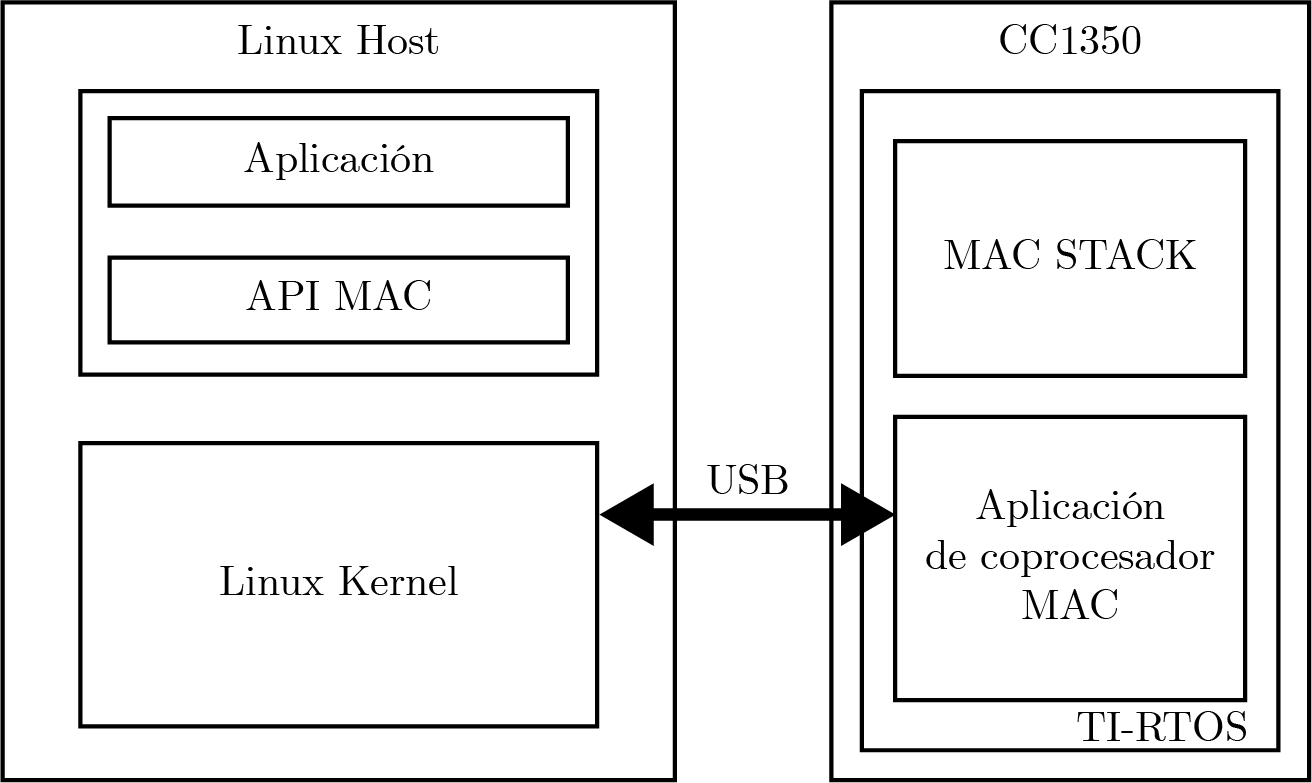
\includegraphics[width=0.8\textwidth]{graphs/concentradorBlockDiagram.png}
	\caption{Arquitectura de software a alto nivel de las aplicaciones TI 15.4-Stack 2.1.0 Linux\R}
	\label{fig:concentradorBlockDiagram}
\end{figure}

Esta secci�n describe la arquitectura de alto nivel basada en coprocesador, los componentes software, y  la arquitectura general del sistema (ve�se figura \ref{fig:concentradorBlockDiagram}). El coprocesador es una entidad que implementa el est�ndar MAC IEEE 802.15.4e/g en un chip dedicado y provee una interfaz serie por la que un procesador externo controla y procesa las operaciones del coprocesador. \\

El concentrador se centra en una arquitectura escalable con una divisi�n perfecta donde el procesador ejecuta las capas sobre el IEEE 802.15.4e/g MAC/PHY.\\

En esta aplicaci�n, el programa se ejecuta en una plataforma basada en Linux. Aunque los componentes de alto nivel , pueden ser conceptualmente aplicados a otras plataformas no basadas en Linux. Los componentes desarrollados ser�n descritos m�s adelante.\\

La interfaz entre el procesador y el coprocesador est�n definidas como capas l�gicas que est�n separadas en esta arquitectura: una capa f�sica (por ejemplo, USB o UART), una capa l�gica de enlace, y la capa de presentaci�n.\\

Componentes software:

\begin{description}
	\item[Aplicaci�n del coprocesador: ] Es el programa ejecutandose en el dispositivo CC1350. Esta aplicaci�n implementa una capa 802.15.4e/g MAC/PHY y proporciona una comunicaci�n serie.
	\item[Kernel Linux]: El kernel Linux provee los controladores para la interfaz serie que est� disponible en un puerto f�sico (por ejemplo, USB).
	\item[Aplicaci�n TI 15.4-Stack: ] Este m�dulo implementa la aplicaci�n usando el protocolo 802.15.4e/g y la estructura del modelo \ac{MT}.
\end{description}

\subsection*{Descripci�n del SDK}
\begin{figure}[h]
	\begin{center}
		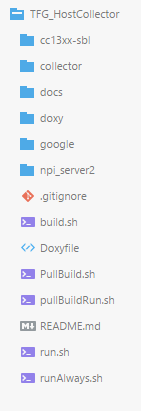
\includegraphics[width=0.5\textwidth]{graphs/fig-oob-dir}
	\end{center}
	\caption{Estructura del directorio TI 15.4-Stack 2.1.0 Linux\R }
	\label{fig:fig-oob-dir}
\end{figure}

La figura \ref{fig:fig-oob-dir} muestra la estructura del directorio de instalaci�n del TI 15.4-Stack 2.1.0. A continuaci�n se explica una descripci�n de alto nivel de cada carpeta:

\begin{description}
	\item[components: ] Contiene las siguientes librer�as:
	\begin{description}
		\item[common: ] Rutinas para caracter�sticas del sistema operativo, como lectura y escritura de ficheros.
		\item[nv: ]  Simula una memoria no vol�til, como la usada en sistemas empotrados.
		\item[api: ] Interfaz de mensajes API MAC y MT
	\end{description}
	\item[docs: ] Documentos como la gu�a de desarrollo y la gu�a de comandos MAC para el coprocesador.
	\item[example: ] Aplicaci�n de ejemplo
	\begin{description}
		\item[cc13xx-sbl: ] Herramientas para la actualizaci�n para los dispositivos CC13x0.
		\item[collector: ]  Aplicaci�n de ejemplo que demuestra como iniciar una red, permitir la conexi�n de dispositivos y recoger datos desde dispositivos remotos.
		\item[gateway: ] Una aplicaci�n basada en Node.js\TM que crea un servidor local y muestra la informaci�n de la red y los datos de los nodos.
		\item[npi\_server2: ] Interfaz socket para comunicarse con el coprocesador.
		\item[google: ] Contiene un makefile para descargar e instalar el compilador de \textit{Google protocol buffer}.
	\end{description}
	\item[firmware] Precompilados ficheros .hex para el coprocesador.
	\item[prebuilt] Compilaci�n para ejecutar la aplicaci�n de ejemplo en una BeagleBone Black.
	\item[scripts] Contiene fragmentos de ficheros makefile usados para compilar la aplicaci�n de ejemplo.
\end{description}

\subsection*{Funcionamiento}

El proyecto comienza en la funci�n \textit{main()}  en el fichero \textit{linux\_main.c}, donde se inicializan las diferentes interfaces, se lee el fichero de configuraci�n y ejecuta la funci�n \textit{App\_main()} del fichero \textit{appsrv.c}.\\

La funci�n \textit{App\_main()} se encarga de inicializar los dos hilos de ejecuci�n principales que tiene el programa, \textit{client-thread} y \textit{collector-thread}. La tarea del cliente se encarga de conectarse al servidor y procesar la transmisi�n y recepci�n de datos por ese canal. Por otro lado la tarea del concentrador, se encarga de generar la red TI 15.4-Stack y procesar los mensajes enviados por este protocolo. \\

\subsubsection*{Hilo del cliente web}
Este hilo mantiene la comunicaci�n con el servidor, y espera recibir un mensaje de este. Cuando un mensaje es recibido la funci�n \textit{appsrv\_handle\_appClient\_request()} es la encargada de procesar el mensaje y notificar a la red TI 15.4-Stack a trav�s del hilo del concentrador.

\subsection*{Hilo del concentrador}

La funci�n \textit{Collector\_process()} del fichero \textit{collector.c} contiene la l�gica de esta tarea, que se describe en la figura ??.

% TODO Incluir figura

\subsection*{Protocol Buffers}

Para facilitar el env�o de datos entre el concentrador y el servidor, se ha utilizado \textit{Protocol Buffers}.\\

\textit{Protocol Buffers} es un mecanismo flexible, eficiente y automatizado para estructurar datos estructurados. Solo es necesario indicar como se estructuran los datos y al compilarse generan la implementaci�n en multiples lenguajes de programaci�n de los mecanismo para codificar y descodificar datos. \\

\subsection*{Funcionamiento}

La estructura de los datos a codificar se definen en archivos .proto. Cada mensaje es una peque�a estructura que contiene una serie de parejas clave-valor. (Ap�ndice \ref{apd:estructurasMensajes} )

Como se observa en el listado \ref{lst:protofield}, el formato de los mensajes es simple y similar a la definici�n de variables en c�digo C. Una vez definidos los mensajes, se ejecuta el compilador de \textit{Protocol Buffers} para el lenguaje de tu aplicaci�n, en nuestro caso C.\\

\lstinputlisting[caption=Ejemplo de estructura con Protocol Buffers,label=lst:protofield,linewidth=\textwidth,breaklines=true,language=C++]{code/Smsgs_msgStatsField.proto}


Las estructuras de datos para nuestra aplicaci�n se pueden observar en el Ap�ndice \ref{apd:estructurasMensajes}. En este podemos observa que hemos creado un fichero con las mismas estructuras a smsgs.h para poder convertir los mensajes que nos llegan de los nodos en mensajes  \textit{Protocol Buffers} y as� poder enviarlos al servidor.





\chapterend{}
